
%%%%%%%%%%%%%%%%%%%%%%%%%%%%%%%%%%%%%%%%%%%%%%%%%%%%%%%%%%%%%%%%%%%%%%%%%%%%%
\chapt[chap:parsers]{Parsers}
\markboth{Parsers}{Parsers}
%%%%%%%%%%%%%%%%%%%%%%%%%%%%%%%%%%%%%%%%%%%%%%%%%%%%%%%%%%%%%%%%%%%%%%%%%%%%%
\nnormalsize

%%%%%%%%%%%%%%%%%%%%%%%%%%%%%%%%%%%%%%%%%%%%%%%%%%%%%%%%%%%%%%%%%%%%%%%%%%%%%
%\sect[sec:parsers:minipar]{MiniPar Parser}
%%%%%%%%%%%%%%%%%%%%%%%%%%%%%%%%%%%%%%%%%%%%%%%%%%%%%%%%%%%%%%%%%%%%%%%%%%%%%
% 
% MiniPar is a shallow parser. In its shipped version, it takes one sentence as an
% input and determines the dependency relationships between the words of a
% sentence. It parses the sentence and brings out the information such as:
% \begin{itemize}
% \item the lemma of the word;
% \item the part of speech of the word;
% \item the head modified by this word;
% \item name of the dependency relationship between this word and the head;
% \item the lemma of the head.
% \end{itemize}
% 
% In the version of MiniPar integrated in GATE (`Parser\_Minipar' plugin), it
% generates annotations of type `DepTreeNode' and the annotations of type
% `[relation]' that exists between the head and the child node. The document is
% required to have annotations of type `Sentence', where each annotation consists
% of a string of the sentence.
% 
% Minipar takes one sentence at a time as an input and generates the tokens of
% type `DepTreeNode'. Later it assigns relation between these tokens. Each
% DepTreeNode consists of feature called `word': this is the actual text of the
% word.
% 
% For each and every annotation of type `[Rel]', where `Rel' is obj, pred etc.
% This is the name of the dependency relationship between the child word and the
% head word (see Section \ref{sec:parsers:minipar:GR}). Every `[Rel]' annotation is assigned four
% features:
% 
% \begin{itemize}
% \item \textbf{child\_word}: this is the text of the child annotation;
% \item \textbf{child\_id}: IDs of the annotations which modify the current word (if any).
% \item \textbf{head\_word}: this is the text of the head annotation;
% \item \textbf{head\_id}: ID of the annotation modified by the child word (if any);
% \end{itemize}
% 
% \begin{figure}[t]
%   \begin{center}
%     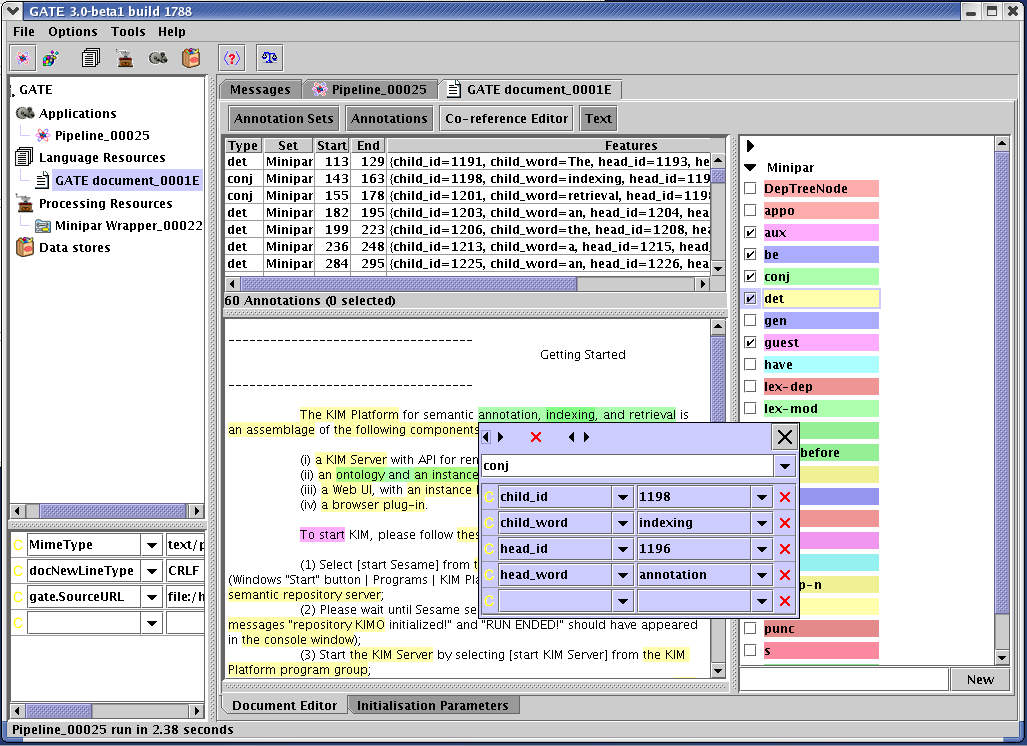
\includegraphics[width=\textwidth]{Minipar.png}
%     \caption{a MiniPar annotated document}
%     \label{fig:minipar}
%   \end{center}
% \end{figure}
% 
% Figure \ref{fig:minipar} shows a MiniPar annotated document in GATE Developer.
% 
% \subsect{Platform Supported}
% 
% MiniPar in GATE is supported for the Linux and Windows operating systems. Trying
% to instantiate this PR on any other OS will generate the
% ResourceInstantiationException.
% 
% \subsect{Resources}
% 
% MiniPar in GATE is shipped with four basic resources:
% \begin{itemize}
% \item
% \textbf{MiniparWrapper.jar}: this is a JAVA Wrapper for MiniPar;
% \item
% \textbf{creole.XML}: this defines the required parameters for MiniPar Wrapper;
% \item
% \textbf{minipar.linux}: this is a modified version of pdemo.cpp.
% \item
% \textbf{minipar-windows.exe} : this is a modified version of pdemo.cpp compiled to work on windows.
% \end{itemize}
% 
% \subsect{Parameters}
% 
% The MiniPar wrapper takes six parameters:
% \begin{itemize}
% \item
% \textbf{annotationTypeName}: new annotations are created with this type, default is "DepTreeNode";
% \item
% \textbf{annotationInputSetName}: annotations of Sentence type are provided as an input to MiniPar and are taken from the given annotationSet;
% \item
% \textbf{annotationOutputSetName}: All annotations created by Minipar Wrapper are stored under the given annotationOutputSet;
% \item
% \textbf{document}: the GATE document to process;
% \item
% \textbf{miniparBinary}: location of the MiniPar Binary file (i.e. either minipar.linux or minipar-windows.exe.  These files are available under gate/plugins/minipar/ directory);
% \item
% \textbf{miniparDataDir}: location of the `data' directory under the installation directory of MINIPAR. default is "\%MINIPAR\_HOME\%/data".
% \end{itemize}
% 
% \subsect{Prerequisites}
% 
% The MiniPar wrapper requires the MiniPar library to be available on the
% underlying Linux/Windows machine. It can be downloaded from the
% \htlink{http://www.cs.ualberta.ca/~lindek/minipar.htm}{MiniPar homepage}.
% 
% \subsect[sec:parsers:minipar:GR]{Grammatical Relationships}
% \begin{small}\begin{verbatim}
% appo    "ACME president, --appo-> P.W. Buckman"
% aux "should <-aux-- resign"
% be  "is <-be-- sleeping"
% c   "that <-c-- John loves Mary"
% comp1   first complement
% det "the <-det `-- hat"
% gen "Jane's <-gen-- uncle"
% i   the relationship between a C clause and its I clause
% inv-aux     inverted auxiliary: "Will <-inv-aux-- you stop it?"
% inv-be      inverted be: "Is <-inv-be-- she sleeping"
% inv-have    inverted have: "Have <-inv-have-- you slept"
% mod the relationship between a word and its adjunct modifier
% pnmod       post nominal modifier
% p-spec      specifier of prepositional phrases
% pcomp-c     clausal complement of prepositions
% pcomp-n     nominal complement of prepositions
% post        post determiner
% pre         pre determiner
% pred        predicate of a  clause
% rel         relative clause
% vrel        passive verb modifier of nouns
% wha, whn, whp:  wh-elements at C-spec positions
% obj         object of verbs
% obj2    second object of ditransitive verbs
% subj    subject of verbs
% s   surface subjec
% \end{verbatim}\end{small}
% 
% 
%%%%%%%%%%%%%%%%%%%%%%%%%%%%%%%%%%%%%%%%%%%%%%%%%%%%%%%%%%%%%%%%%%%%%%%%%%%%%
\sect[sec:parsers:rasp]{RASP Parser}
%%%%%%%%%%%%%%%%%%%%%%%%%%%%%%%%%%%%%%%%%%%%%%%%%%%%%%%%%%%%%%%%%%%%%%%%%%%%%
RASP (Robust Accurate Statistical Parsing) is a robust parsing system
for English, developed by the Natural Language and Computational
Linguistics group at the University of Sussex.

This plugin, `Parser\_RASP', developed by
\htlink{http://www.digitalpebble.com/}{DigitalPebble}, provides four
wrapper PRs that call the RASP modules as external programs, as well
as a JAPE component that translates the output of the ANNIE POS Tagger
(Section~\ref{sec:annie:tagger}).
%
\begin{description}
\item[RASP2 Tokenizer] This PR requires \texttt{Sentence} annotations
  and creates \texttt{Token} annotations with a \texttt{string}
  feature.  Note that sentence-splitting must be carried out before
  tokenization; the the RegEx Sentence Splitter (see
  Section~\ref{sec:annie:regex-splitter}) is suitable for this.
  (Alternatively, you can use the ANNIE Tokenizer
  (Section~\ref{sec:annie:tokeniser}) and then the ANNIE Sentence Splitter
  (Section~\ref{sec:annie:splitter}); their output is compatible with the
  other PRs in this plugin).
\item[RASP2 POS Tagger] This requires \texttt{Token} annotations and
  creates \texttt{WordForm} annotations with \texttt{pos},
  \texttt{probability}, and \texttt{string} features.
\item[RASP2 Morphological Analyser] This requires \texttt{WordForm}
  annotations (from the POS Tagger) and adds \texttt{lemma} and
  \texttt{suffix} features.
\item[RASP2 Parser] This requires the preceding annotation types and
  creates multiple \texttt{Dependency} annotations to represent a
  parse of each sentence.
\item[RASP POS Converter] This PR requires \texttt{Token} annotations
  with a \texttt{category} feature as produced by the ANNIE POS Tagger
  (see Section~\ref{sec:annie:tagger} and creates \texttt{WordForm}
  annotations in the RASP Format.  The ANNIE POS Tagger and this
  Converter can together be used as a substitute for the RASP2 POS
  Tagger.
\end{description}


Here are some examples of corpus pipelines that can be correctly
constructed with these PRs.
\begin{enumerate}
\item RegEx Sentence Splitter
\item RASP2 Tokenizer
\item RASP2 POS Tagger
\item RASP2 Morphological Analyser
\item RASP2 Parser
\end{enumerate}
%
\begin{enumerate}
\item RegEx Sentence Splitter
\item RASP2 Tokenizer
\item ANNIE POS Tagger
\item RASP POS Converter
\item RASP2 Morphological Analyser
\item RASP2 Parser
\end{enumerate}
%
\begin{enumerate}
\item ANNIE Tokenizer
\item ANNIE Sentence Splitter
\item RASP2 POS Tagger
\item RASP2 Morphological Analyser
\item RASP2 Parser
\end{enumerate}
%
\begin{enumerate}
\item ANNIE Tokenizer
\item ANNIE Sentence Splitter
\item ANNIE POS Tagger
\item RASP POS Converter
\item RASP2 Morphological Analyser
\item RASP2 Parser
\end{enumerate}




Further documentation is included in the directory
\verb!gate/plugins/Parser\_RASP/doc/!.


The RASP package, which provides the external programs, is available
from the
\htlink{http://www.informatics.sussex.ac.uk/research/groups/nlp/rasp/}{RASP
  web page}.

RASP is only supported for Linux operating systems. Trying to run it
on any other operating systems will generate an exception with the
message: `The RASP cannot be run on any other operating systems
except Linux.'

It must be correctly installed on the same machine as GATE, and must
be installed in a directory whose path does not contain any spaces
(this is a requirement of the RASP scripts as well as the
wrapper). Before trying to run scripts for the first time, edit
\verb!rasp.sh! and \verb!rasp_parse.sh! to set the correct value
for the shell variable RASP, which should be the file system pathname
where you have installed the RASP tools (for example,
\texttt{RASP=/opt/RASP} or \texttt{RASP=/usr/local/RASP}.  You will
need to enter the same path for the initialization parameter
\texttt{raspHome} for the POS Tagger, Morphological Analyser, and
Parser PRs.

(On some systems the \texttt{arch} command used in the scripts is not
available; a work-around is to comment that line out and add
\verb!arch='ix86_linux'!, for example.)


(The previous version of the RASP plugin can now be found in
\verb!plugins/Obsolete/rasp!.)
%
%
%%%%%%%%%%%%%%%%%%%%%%%%%%%%%%%%%%%%%%%%%%%%%%%%%%%%%%%%%%%%%%%%%%%%%%%%%%%%%
\sect[sec:parsers:supple]{SUPPLE Parser}
%%%%%%%%%%%%%%%%%%%%%%%%%%%%%%%%%%%%%%%%%%%%%%%%%%%%%%%%%%%%%%%%%%%%%%%%%%%%%
% add the old label and HTML anchor, for backwards compatibility
\label{sec:parsers:buchart}\htcode{<A NAME="sec:parsers:buchart"></A>}

SUPPLE is a bottom-up parser that constructs syntax trees and logical forms for
English sentences. The parser is complete in the sense that every analysis
licensed by the grammar is produced. In the current version only the `best'
parse is selected at the end of the parsing process. The English grammar is
implemented as an attribute-value context free grammar which consists of
subgrammars for noun phrases (NP), verb phrases (VP), prepositional phrases
(PP), relative phrases (R) and sentences (S). The semantics associated with each
grammar rule allow the parser to produce logical forms composed of unary
predicates to denote entities and events (e.g., {\em chase(e1)}, {\em run(e2)})
and binary predicates for properties (e.g. {\em lsubj(e1,e2)}). Constants (e.g.,
$e1$, $e2$) are used to represent entity and event identifiers. The GATE SUPPLE
Wrapper stores syntactic information produced by the parser in the gate document
in the form of \texttt{parse} annotations containing a bracketed
representation of the parse; and \texttt{semantics} annotations that contains
the logical forms produced by the parser.  It also produces
\texttt{SyntaxTreeNode} annotations that allow viewing of the parse tree for a
sentence (see Section~\ref{sec:parsers:supple:treeviewer}).

%%%%%%%%%%%%%%%%%%%%%%%%%%%%%%%%%%%%%%%%%%%%%%%%%%%%%%%%%%%%%%%%%%%%%%%%%%%%%
\subsect{Requirements}
%%%%%%%%%%%%%%%%%%%%%%%%%%%%%%%%%%%%%%%%%%%%%%%%%%%%%%%%%%%%%%%%%%%%%%%%%%%%%

The SUPPLE parser is written in Prolog, so you will need a Prolog interpreter
to run the parser.  A copy of PrologCafe
(\htlinkplain{http://kaminari.scitec.kobe-u.ac.jp/PrologCafe/}), a pure Java
Prolog implementation, is provided in the distribution.  This should work on
any platform but it is not particularly fast.  SUPPLE also supports the
open-source SWI Prolog (\htlinkplain{http://www.swi-prolog.org}) and the
commercially licenced SICStus prolog
(\htlinkplain{http://www.sics.se/sicstus}, SUPPLE supports versions 3 and 4),
which are available for Windows, Mac OS X, Linux and other Unix variants.  For
anything more than the simplest cases we recommend installing one of these
instead of using PrologCafe.

%%%%%%%%%%%%%%%%%%%%%%%%%%%%%%%%%%%%%%%%%%%%%%%%%%%%%%%%%%%%%%%%%%%%%%%%%%%%%
\subsect{Building SUPPLE}
%%%%%%%%%%%%%%%%%%%%%%%%%%%%%%%%%%%%%%%%%%%%%%%%%%%%%%%%%%%%%%%%%%%%%%%%%%%%%

The SUPPLE plugin must be compiled before it can be used, so you will require a
suitable Java SDK (GATE itself requires only the JRE to run). To build SUPPLE,
first edit the file {\tt build.xml} in the {\tt Parser\_SUPPLE} directory under
{\tt plugins}, and adjust the user-configurable options at the top of the file to
match your environment.  In particular, if you are using SWI or SICStus Prolog,
you will need to change the {\tt swi.executable} or {\tt sicstus.executable}
property to the correct name for your system. Once this is done, you can build
the plugin by opening a command prompt or shell, going to the {\tt Parser\_SUPPLE}
directory and running:
\begin{small}\begin{verbatim}
ant swi
\end{verbatim}\end{small}
For PrologCafe or SICStus, replace {\tt swi} with {\tt plcafe} or {\tt sicstus} as
appropriate.

%%%%%%%%%%%%%%%%%%%%%%%%%%%%%%%%%%%%%%%%%%%%%%%%%%%%%%%%%%%%%%%%%%%%%%%%%%%%%
\subsect{Running the Parser in GATE}
%%%%%%%%%%%%%%%%%%%%%%%%%%%%%%%%%%%%%%%%%%%%%%%%%%%%%%%%%%%%%%%%%%%%%%%%%%%%%

In order to parse a document you will need to construct an application that has:

\begin{itemize}

\item tokeniser

\item splitter

\item POS-tagger

\item Morphology

\item SUPPLE Parser with parameters

\subitem mapping file (config/mapping.config)
\subitem feature table file (config/feature\_table.config)
\subitem parser file (supple.plcafe or supple.sicstus or
supple.swi)
\subitem prolog implementation (shef.nlp.supple.prolog.PrologCafe,\\
shef.nlp.supple.prolog.SICStusProlog3, shef.nlp.supple.prolog.SICStusProlog4,\\
shef.nlp.supple.prolog.SWIProlog or
shef.nlp.supple.prolog.SWIJavaProlog\footnote{shef.nlp.supple.prolog.SICStusProlog
exists for backwards compatibility and behaves the same as SICStusProlog3.}).

You can take a look at build.xml to see examples of invocation for
the different implementations.

\end{itemize}

\textbf{Note} that prior to GATE 3.1, the parser file parameter was of type
\texttt{java.io.File}.  From 3.1 it is of type \texttt{java.net.URL}.  If you
have a saved application (.gapp file) from before GATE 3.1 which includes
SUPPLE it will need to be updated to work with the new version.  Instructions
on how to do this can be found in the README file in the SUPPLE plugin
directory.


%%%%%%%%%%%%%%%%%%%%%%%%%%%%%%%%%%%%%%%%%%%%%%%%%%%%%%%%%%%%%%%%%%%%%%%%%%%%%
\subsect[sec:parsers:supple:treeviewer]{Viewing the Parse Tree}
%%%%%%%%%%%%%%%%%%%%%%%%%%%%%%%%%%%%%%%%%%%%%%%%%%%%%%%%%%%%%%%%%%%%%%%%%%%%%

GATE Developer provides a syntax tree viewer in the \texttt{Tools} plugin which
can display the parse tree generated by SUPPLE for a sentence.  To use the tree
viewer, be sure that the \texttt{Tools} plugin is loaded, then open a document in
GATE Developer that has been processed with SUPPLE and view its \texttt{Sentence}
annotations.  Right-click on the relevant \texttt{Sentence} annotation in the
annotations table and select `Edit with syntax tree viewer'.  This viewer can
also be used with the constituency output of the Stanford Parser PR
(Section~\ref{sec:parsers:stanford}).


%%%%%%%%%%%%%%%%%%%%%%%%%%%%%%%%%%%%%%%%%%%%%%%%%%%%%%%%%%%%%%%%%%%%%%%%%%%%%
\subsect[sec:parsers:supple:properties]{System Properties}
%%%%%%%%%%%%%%%%%%%%%%%%%%%%%%%%%%%%%%%%%%%%%%%%%%%%%%%%%%%%%%%%%%%%%%%%%%%%%

The \texttt{SICStusProlog} (3 and 4) and \texttt{SWIProlog} implementations
work by calling the native prolog executable, passing data back and forth in
temporary files.  The location of the prolog executable is specified by a
system property:
%
\begin{itemize}
\item for SICStus: \texttt{supple.sicstus.executable} - default is to look for
\texttt{sicstus.exe} (Windows) or \texttt{sicstus} (other platforms) on the
PATH.
\item for SWI: \texttt{supple.swi.executable} - default is to look for
\texttt{plcon.exe} (Windows) or \texttt{swipl} (other platforms) on the PATH.
\end{itemize}

If your prolog is installed under a different name, you should specify the
correct name in the relevant system property.  For example, when installed from
the source distribution, the Unix version of SWI prolog is typically installed
as \texttt{pl}, most binary packages install it as \texttt{swipl}, though some
use the name \texttt{swi-prolog}.  You can also use the properties to specify
the full path to prolog (e.g. \texttt{/opt/swi-prolog/bin/pl}) if it is not on
your default PATH.

For details of how to pass system properties to GATE, see
the end of Section \ref{sec:gettingstarted:sysprop}.

\subsect[sec:supple:config]{Configuration Files}

Two files are used to pass information from GATE to the SUPPLE
parser: the {\em mapping} file and the {\em feature table} file.\\

%%%%%%%%%%%%%%%%%%%%%%%%%%%%%%%%%%%%%%%%%%%%%%%%%%%%%%%%%%%%%%%%%%%%%%%%%%%%%
\subsubsect{Mapping File}
%%%%%%%%%%%%%%%%%%%%%%%%%%%%%%%%%%%%%%%%%%%%%%%%%%%%%%%%%%%%%%%%%%%%%%%%%%%%%

The mapping file specifies how annotations produced using GATE are to be passed
to the parser. The file is composed of a number of pairs of lines, the first
line in a pair specifies a GATE annotation we want to pass to the parser. It
includes the AnnotationSet (or default), the AnnotationType, and a number of
features and values that depend on the AnnotationType. The second line of the
pair specifies how to encode the GATE annotation in a SUPPLE syntactic
category, this line also includes a number of features and values. As an example
consider the mapping:

\begin{small}\begin{verbatim}
Gate;AnnotationType=Token;category=DT;string=&S
SUPPLE;category=dt;m_root=&S;s_form=&S
\end{verbatim}\end{small}


It specifies how a determinant ('DT') will be translated into a category `dt'
for the parser. The construct `\&S' is used to represent a variable that will be
instantiated to the appropriate value during the mapping process. More
specifically a token like `The' recognised as a DT by the POS-tagging will be
mapped into the following category:

\begin{small}\begin{verbatim}
dt(s_form:'The',m_root:'The',m_affix:'_',text:'_').
\end{verbatim}\end{small}


As another example consider the mapping:

\begin{small}\begin{verbatim}
Gate;AnnotationType=Lookup;majorType=person_first;minorType=female;string=&S
SUPPLE;category=list_np;s_form=&S;ne_tag=person;ne_type=person_first;gender=female
\end{verbatim}\end{small}


It specified that an annotation of type `Lookup' in GATE is mapped into a
category `list\_np' with specific features and values. More specifically a token
like `Mary' identified in GATE as a Lookup will be mapped into the following
SUPPLE category:

\begin{small}\begin{verbatim}
list_np(s_form:'Mary',m_root:'_',m_affix:'_',
text:'_',ne_tag:'person',ne_type:'person_first',gender:'female').
\end{verbatim}\end{small}



%%%%%%%%%%%%%%%%%%%%%%%%%%%%%%%%%%%%%%%%%%%%%%%%%%%%%%%%%%%%%%%%%%%%%%%%%%%%%
\subsubsect[sec:parsers:supple:features]{Feature Table}
%%%%%%%%%%%%%%%%%%%%%%%%%%%%%%%%%%%%%%%%%%%%%%%%%%%%%%%%%%%%%%%%%%%%%%%%%%%%%

The feature table file specifies SUPPLE `lexical' categories and its
features.  As an example an entry in this file is:

\begin{small}\begin{verbatim}
n;s_form;m_root;m_affix;text;person;number
\end{verbatim}\end{small}


which specifies which features and in which order a noun category
should be written. In this case:

\begin{small}\begin{verbatim}
n(s_form:...,m_root:...,m_affix:...,text:...,person:...,number:....).
\end{verbatim}\end{small}

%%%%%%%%%%%%%%%%%%%%%%%%%%%%%%%%%%%%%%%%%%%%%%%%%%%%%%%%%%%%%%%%%%%%%%%%%%%%%
\subsect[sec:parsers:supple:grammar]{Parser and Grammar}
%%%%%%%%%%%%%%%%%%%%%%%%%%%%%%%%%%%%%%%%%%%%%%%%%%%%%%%%%%%%%%%%%%%%%%%%%%%%%

The parser builds a semantic representation compositionally, and a `best parse'
algorithm is applied to each final chart, providing a partial parse if no
complete sentence span can be constructed. The parser uses a feature valued
grammar. Each \texttt{Category} entry has the form:
\begin{small}\begin{verbatim}
Category(Feature1:Value1,...,FeatureN:ValueN)
\end{verbatim}\end{small}
where the number and type of features is dependent on the category
type (see Section ~\ref{sec:corpora:features}).  All categories will have the features \texttt{s\_form} (surface
form) and \texttt{m\_root} (morphological root); nominal and verbal
categories will also have \texttt{person} and \texttt{number}
features; verbal categories will also have \texttt{tense} and
\texttt{vform} features; and adjectival categories will have a
\texttt{degree} feature.  The \texttt{list\_np} category has the same
features as other nominal categories plus \texttt{ne\_tag} and
\texttt{ne\_type}.

Syntactic rules are specified in Prolog with the predicate
$rule(LHS,RHS)$ where $LHS$ is a syntactic category and
$RHS$ is a list of syntactic categories. A rule such as $BNP\_HEAD
\Rightarrow N$ (`a basic noun phrase head is composed of a noun') is
written as follows:

\begin{small}\begin{verbatim}
rule(bnp_head(sem:E^[[R,E],[number,E,N]],number:N),
[n(m_root:R,number:N)]).
\end{verbatim}\end{small}
where the feature `sem' is used to construct the semantics while the parser
processes input, and E, R, and N are variables to be instantiated during parsing.

The full grammar of this distribution can be found in the prolog/grammar
directory, the file load.pl specifies which grammars are used by the parser. The
grammars are compiled when the system is built and the compiled version is used
for parsing.

%%%%%%%%%%%%%%%%%%%%%%%%%%%%%%%%%%%%%%%%%%%%%%%%%%%%%%%%%%%%%%%%%%%%%%%%%%%%%
\subsect{Mapping Named Entities}
%%%%%%%%%%%%%%%%%%%%%%%%%%%%%%%%%%%%%%%%%%%%%%%%%%%%%%%%%%%%%%%%%%%%%%%%%%%%%

SUPPLE has a prolog grammar which deals with named entities, the only
information required is the Lookup annotations produced by Gate, which are
specified in the mapping file. However, you may want to pass named entities
identified with your own Jape grammars in GATE. This can be done using a special
syntactic category provided with this distribution. The category sem\_cat is
used as a bridge between Gate named entities and the SUPPLE grammar. An example
of how to use it (provided in the mapping file) is:

\begin{small}\begin{verbatim}
Gate;AnnotationType=Date;string=&S
SUPPLE;category=sem_cat;type=Date;text=&S;kind=date;name=&S
\end{verbatim}\end{small}
which maps a named entity `Date' into a syntactic  category
'sem\_cat'.  A grammar file called semantic\_rules.pl is provided
to map sem\_cat into the appropriate  syntactic category expected by
the phrasal rules. The following rule for example:
\begin{small}\begin{verbatim}
rule(ne_np(s_form:F,sem:X^[[name,X,NAME],[KIND,X]]),[
sem_cat(s_form:F,text:TEXT,type:'Date',kind:KIND,name:NAME)]).
\end{verbatim}\end{small}
is used to parse a `Date' into a named entity in SUPPLE which in turn
will be parsed into a noun phrase.

%%%%%%%%%%%%%%%%%%%%%%%%%%%%%%%%%%%%%%%%%%%%%%%%%%%%%%%%%%%%%%%%%%%%%%%%%%%%%
\subsect{Upgrading from BuChart to SUPPLE}
%%%%%%%%%%%%%%%%%%%%%%%%%%%%%%%%%%%%%%%%%%%%%%%%%%%%%%%%%%%%%%%%%%%%%%%%%%%%%

In theory upgrading from BuChart to SUPPLE should be relatively straightforward.
Basically any instance of BuChart needs to be replaced by SUPPLE. Specific changes
which must be made are:

\begin{itemize}
\item The compiled parser files are now supple.swi, supple.sicstus, or supple.plcafe
\item The GATE wrapper parameter buchartFile is now SUPPLEFile, and it is now
of type {\tt java.net.URL} rather than {\tt java.io.File}.  Details of how to
compensate for this in existing saved applications are given in the SUPPLE
README file.
\item The Prolog wrappers now start shef.nlp.supple.prolog instead of shef.nlp.buchart.prolog
\item The mapping.conf file now has lines starting SUPPLE; instead of Buchart;
\item Most importantly the main wrapper class is now called nlp.shef.supple.SUPPLE
\end{itemize}

Making these changes to existing code should be trivial and allow application
to benefit from future improvements to SUPPLE.
%%%%%
%%%%%
%%%%%%%%%%%%%%%%%%%%%%%%%%%%%%%%%%%%%%%%%%%%%%%%%%%%%%%%%%%%%%%%%%%%%%%%%%%%%
\sect[sec:parsers:stanford]{Stanford Parser}
%%%%%%%%%%%%%%%%%%%%%%%%%%%%%%%%%%%%%%%%%%%%%%%%%%%%%%%%%%%%%%%%%%%%%%%%%%%%%
%%%%%
The \htlink{http://nlp.stanford.edu/software/lex-parser.shtml}{Stanford Parser}
is a probabilistic parsing system implemented in Java by Stanford University's
\htlink{http://nlp.stanford.edu/}{Natural Language Processing Group}.  Data
files are available from Stanford for parsing Arabic, Chinese, English, and
German.


This PR (\texttt{gate.stanford.Parser}) acts as a wrapper around the Stanford
Parser and translates GATE annotations to and from the data
structures of the parser itself.  The plugin is supplied with the unmodified
\texttt{jar} file and one English data file obtained from Stanford.  Stanford's
software itself is subject to the full GPL.


The parser itself can be trained on other corpora and languages, as documented
on the \htlink{http://nlp.stanford.edu/software/lex-parser.shtml}{website}, but
this plugin does not provide a means of doing so.  Trained data files are not
necessarily compatible between different versions of the parser.

The current versions of the Stanford parser and this PR are threadsafe.
Multiple instances of the PR with the same or different model files can be used
simultaneously.
%
%%%%%%%%%%%%%%%%%%%%%%%%%%%%%%%%%%%%%%%%%%%%%%%%%%%%%%%%%%%%%%%%%%%%%%%%%%%%%
\subsect{Input Requirements}
%%%%%%%%%%%%%%%%%%%%%%%%%%%%%%%%%%%%%%%%%%%%%%%%%%%%%%%%%%%%%%%%%%%%%%%%%%%%%
%
Documents to be processed by the Parser PR must already have
\texttt{Sentence} and \texttt{Token} annotations, such as those
produced by either ANNIE Sentence Splitter
(Sections~\ref{sec:annie:splitter} and~\ref{sec:annie:regex-splitter}) and the
ANNIE English Tokeniser (Section~\ref{sec:annie:tokeniser}).

If the \texttt{reusePosTags} parameter is true, then the
\texttt{Token} annotations must have \texttt{category} features with
compatible POS tags.  The tags produced by the ANNIE POS Tagger are
compatible with Stanford's parser data files for English (which also
use the Penn treebank tagset).
%
\subsect{Initialization Parameters}
\begin{description}
%
\item[parserFile] the path to the trained data file; the default value
  points to the English data
  file\footnote{\texttt{resources/englishPCFG.ser.gz}} included with
  the GATE distribution.  You can also use other files downloaded from
  the
  \htlink{http://nlp.stanford.edu/software/lex-parser.shtml}{Stanford
    Parser} website or produced by training the parser.
%
\item[mappingFile] the optional path to a mapping file: a flat,
  two-column file which the wrapper can use to `translate' tags.  A
  sample file is
  included.\footnote{\texttt{resources/english-tag-map.txt}} By
  default this value is \texttt{null} and mapping is ignored.
%
\item[tlppClass] an implementation of
  \texttt{TreebankLangParserParams}, used by the parser itself to
  extract the dependency relations from the constituency structures.
  The default value is compatible with the English data file supplied.
  Please refer to the Stanford NLP Group's documentation and the
  parser's javadoc for a further explanation.
%
\end{description}
%
\subsect{Runtime Parameters}
\begin{description}
\item[annotationSetName] the name of the annotationSet used for input (\texttt{Token} and
  \texttt{Sentence} annotations) and output (\texttt{SyntaxTreeNode}
  and \texttt{Dependency} annotations, and \texttt{category} and
  \texttt{dependencies} features added to \texttt{Tokens}).
\item[debug] a boolean value which controls the verbosity of the
  wrapper's output.
\item[reusePosTags] if true, the wrapper will read \texttt{category}
  features (produced by an earlier POS-tagging PR) from the
  \texttt{Token} annotations and force the parser to use them.
\item[useMapping] if this is true and a mapping file was loaded when
  the PR was initialized, the POS and syntactic tags produced by the
  parser will be translated using that file.  If no mapping file was
  loaded, this parameter is ignored.
\end{description}


The following boolean parameters switch on and off the various types
of output that the parser can produce.  Any or all of them can be
true, but if all are false the PR will simply print a warning to save
time (instead of running the parser).
%
\begin{description}
%
\item[addPosTags] if this is true, the wrapper will add
  \texttt{category} features to the \texttt{Token} annotations.
%
\item[addConstituentAnnotations] if true, the wrapper will mark the
  syntactic constituents with \texttt{SyntaxTreeNode} annotations that
  are compatible with the Syntax Tree Viewer (see
  Section~\ref{sec:parsers:supple:treeviewer}).
%
\item[addDependencyAnnotations] if true, the wrapper will add
  \texttt{Dependency} annotations to indicate the dependency relations
  in the sentence.
%
\item[addDependencyFeatures] if true, the wrapper will add
  \texttt{dependencies} features to the \texttt{Token} annotations to 
  indicate the dependency relations in the sentence.
%
\end{description}
%
The parser will derive the dependency structures only if at least one of the
dependency output options is enabled, so if you do not need the dependency
analysis, set both of them to false so the PR will run faster.



The following parameters control the Stanford parser's options for processing
dependencies; please refer to the \emph{Stanford Dependencies
  Manual}\footnote{\url{http://nlp.stanford.edu/software/parser-faq.shtml}} for
details.  These parameters are ignored unless at least one of the
dependency-related parameters above is true.  The default values (\texttt{Typed}
and \texttt{false}) correspond to the behaviour of previous version of this PR.
%%
\begin{description}
%
\item[dependencyMode] One of the following values:
%
  \begin{tabular}{ll}
    Mode & equivalent command-line option\\
    \hline
    \texttt{Typed} & \texttt{-basic}\\
    \texttt{AllTyped} & \texttt{-nonCollapsed}\\
    \texttt{TypedCollapsed} & \texttt{-collapsed}\\
    \texttt{TypedCCprocessed} & \texttt{-CCprocessed}    
  \end{tabular}
%
\item[includeExtraDependencies] This has no effect with the \texttt{AllTyped}
  mode; for the others, it determines whether to include ``extras'' such as
  control dependencies; if they are included, the complete set of dependencies
  may not follow a tree structure.
%
\end{description}



Two sample GATE applications for English are included in the
\texttt{plugins/Parser\_Stanford} directory: \verb!sample_parser_en.gapp! runs
the Regex Sentence Splitter and ANNIE Tokenizer and then uses this PR to
annotate POS tags and constituency and dependency structures, whereas
\verb!sample_pos+parser_en.gapp! also runs the ANNIE POS Tagger and makes the
parser re-use its POS tags.
%%%%%%%%%%%%%%%%%%%%%%%%%%%%%%%%%%%%%%%%%%%%%%%%%%
